\documentclass{article}
\usepackage{graphicx}
\usepackage{amsmath,amsthm,amssymb}
\usepackage{epsf}
\usepackage{color}
\newtheorem{theorem}{Theorem}
\setlength{\topmargin}{0.1in}
\setlength{\oddsidemargin}{0in}
\setlength{\evensidemargin}{0in}
\setlength{\headheight}{0in}
\setlength{\headsep}{0in}
\setlength{\textheight}{9in}
\setlength{\textwidth}{6.5in}
\renewcommand{\dblfloatpagefraction}{0.9}
\renewcommand{\floatpagefraction}{0.9}
\newenvironment{bibparagraph}{\begin{list}{}{ %
    \setlength{\labelsep}{-\leftmargin} %
    \setlength{\labelwidth}{0pt} %
    \setlength{\itemindent}{-\leftmargin} %
    \setlength{\listparindent}{0pt}}}{\end{list}}
\def\makefigure#1#2{\begin{figure}
\begin{center}
\input{#1}
\end{center}
\caption{#2}
\label{#1}
\end{figure}}

\def\limplies{\; \supset \;}
\def\land{\: \wedge \:}
\def\lor{\: \vee \:}
\def\iff{\; \equiv \;}
\def\lnot{\neg}
\def\lforall#1{\forall \: #1 \;}
\def\lexists#1{\exists \: #1 \;}
\def\glitch#1{{\tt #1}} % glitch on
%\def\glitch#1{} % glitch off
\def\comment#1{}
\def\pnil{[\;]}
\def\pif{\; \mbox{\tt :- } \;}
\def\tuple#1{$\langle #1\rangle$}
\def\mtuple#1{\langle #1\rangle}
\def\ceiling#1{\lceil #1\rceil}
\def\floor#1{\lfloor #1\rfloor}
\def\centerps#1{\begin{center}
\leavevmode
\epsfbox{#1}
\end{center}}
\def\argmax{\mathop{\rm argmax}}
\def\argmin{\mathop{\rm argmin}}
\def\grad{\nabla\!}
\def\celsius{^\circ\mbox{C}}
%\long\def\answer#1{}  % comment out for solutions
%\long\def\question#1{#1} % comment out for solutions
\long\def\answer#1{{\color {blue} { #1}}}  % comment in for solution
\long\def\question#1{} % comment in for solution

\newcommand{\mb}[1]{{\mathbf{#1}}}
\newcommand{\msb}[1]{{\boldsymbol{#1}}}

\def\z{{\bf z}}
\def\x{{\bf x}}
\def\w{{\bf w}}

\begin{document}
{
\small
Submitted by: {Oluwasegun Somefun}, somefuno@oregonstate.edu
}
{\Large
\begin{center}
AI534 --- Written Homework Assignment 3 (40 pts) --- {Due Nov 12th, 2021}
\end{center}
}
%Please submit via TEACH electronically.
\begin{enumerate}
\item Apply linear SVM without soft margin to the following problem.
\begin{center}
\begin{figure}[h]
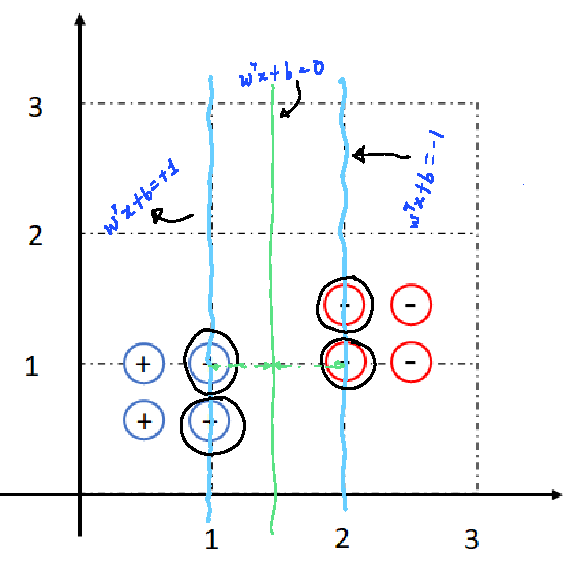
\includegraphics[width=3in]{svm.pdf}
\end{figure}
\end{center}

\begin{itemize} \item[a.] (2pts) Please mark out the support vectors, the decision boundary ($\textbf{w}^T\textbf{x} +b =0$) and $\textbf{w}^T\textbf{x} +b =1$ and $\textbf{w}^T\textbf{x} +b =-1$. Note that you don't need to solve the optimization problem for this, just eyeball the solution.

\answer{
    The support vectors are circled in black ink, and the  decision boundaries are clearly marked out in  Figure~\ref{fig:1}
    \begin{figure}[h]
        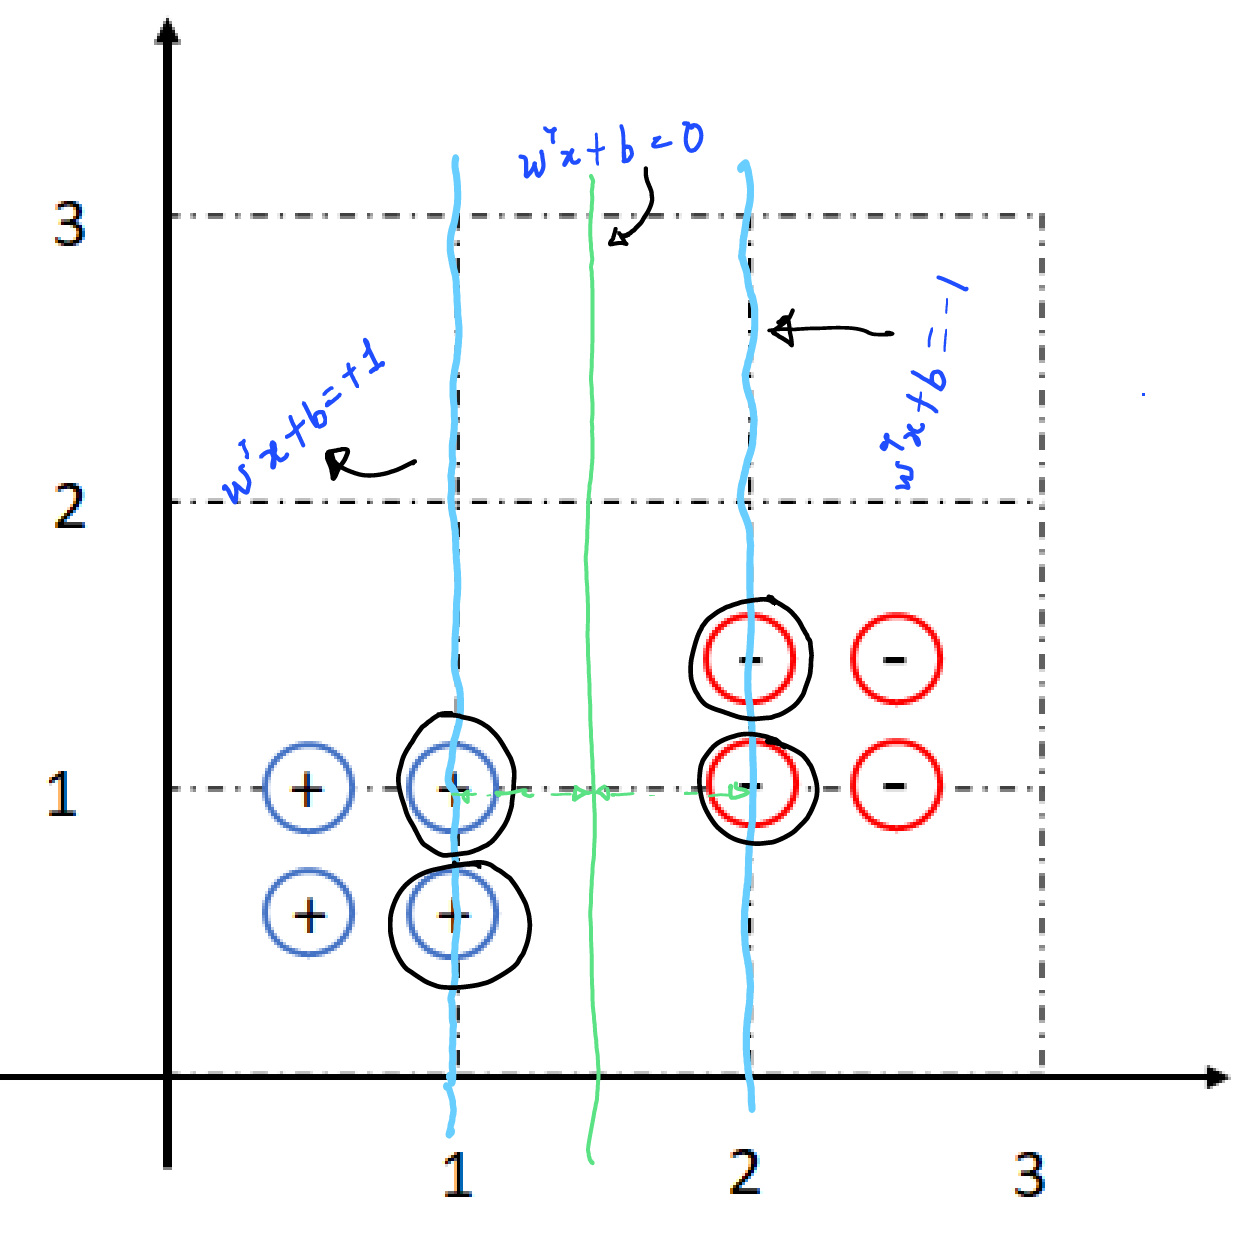
\includegraphics[width=3in]{svm.png}
        \label{fig:1}
        \caption{Marked SVM Decision Boundary}
    \end{figure}
    The support vectors, that can be observed for $\x = (\x_1,\x_2)$ are points on the decision boundary, For the $y = +1$ class, they are potentially  $ \x = (1,1), (1,0.5)$, and for the $y = -1$ class, we have $\x = (2,1), (2,1.5)$

    The exact support vectors with the smallest margin are  $ \x = (1,1),  (2,1)$.

    The decision boundary $\w^T\x + b = 0$ is the vertical straight-line passing through $\x = (1.5,0)$.

    The decision boundary $\w^T\x + b = +1$ is the vertical straight-line passing through $\x = (1,0)$.

    The decision boundary $\w^T\x + b = -1$ is the vertical straight-line passing through $\x = (2,0)$.
}
\item[b.] (6 pts) Please solve for $\textbf{w}$ and $b$ based on the support vectors you identified in (a).

\answer{
    The exact decision boundary line for the half-space is $\w^T\x + b = 0$, which passes through $\x = (1.5,0)$. Solving, we have:

    $$ 
        \left(\begin{matrix}
        b \\ \w_1\\ \w_2 
    \end{matrix}
        \right) 
        \left(\begin{matrix}
            1 \\ \x_1\\ \x_2
        \end{matrix}
            \right) = 
        \left(\begin{matrix}
                b \\ \w_1\\ \w_2 
        \end{matrix}
        \right) 
        \left(\begin{matrix}
         1 \\ 1.5\\ 0
        \end{matrix}
            \right)  = 0
    $$
    $$
        b = -1.5\w_1
    $$
    For each halfspace, supported by  the vectors $\x = (1,1),  (2,1)$ we have:
    $$
        \left(\begin{matrix}
            -1.5\w_1 \\ \w_1\\ \w_2 
        \end{matrix}
            \right) 
            \left(\begin{matrix}
                1 \\ 1\\ 1
            \end{matrix}
                \right) = 1 \quad \hbox{and }
            \left(\begin{matrix}
                   -1.5\w_1 \\ \w_1\\ \w_2 
            \end{matrix}
            \right) 
            \left(\begin{matrix}
             1 \\ 2\\ 1
            \end{matrix}
                \right)  = -1
    $$
    Solving the resulting simultaenous equation we obtain $\w_1 = -2, \w_2 =0, b = 3$ and hence
    $$
        \w = (-2, 0)\quad\hbox{and}\quad b = 3
    $$
}
\end{itemize}

\item $L_2$ SVM\\
Given a set of training examples $\{(\x_i, y_i)\}_{i=1}^N$, where $y_i\in \{1, -1\}$ for all $i$. The following is the primal formulation of $L_2$ SVM, a variant of the standard SVM obtained by squaring the hinge loss:
\begin{align*}
\min_{\w, b, \xi} \mbox{ }& \w^T\w+\lambda\sum_{i=1}^N \xi_i^2 \\
\mbox{s.t. } & y_i(\w^T\x_i+b)\geq 1-\xi_i \mbox{,   } i \in \{1,\cdots,N\}\\
 & \xi_i\geq 0, \mbox{  }  i\in \{1,\cdots,N\}
\end{align*}

\begin{itemize}
\item [a.] (5pts) Show that removing the second constraint $\xi_i\geq 0$ will not change the solution to the problem. In other words, let $(\w^*, b^*, {\bf \xi}^*)$ be the optimal solution to the problem without this set of constraints, show that  ${\bf \xi}_i^* \geq 0$, $\forall i\in\{1,\cdots,N\} $. ( Hint: use proof by contradiction.)\\
\answer{
    \begin{proof}[Proof by Contradiction]
        Assume for some $i \,\,\exists \,\,\xi_i^* < 0$, then the first constraint is satisfied and reduces to:
        $y_i(\w^{*T}\x_i+b)\geq 1 $ which  means there is a point outside the margin that does not contribute to the loss.
        If instead $\xi_i^* = 0$, the first constraint still satisfied reduces to:
        $y_i(\w^{*T}\x_i+b)\geq 1 $ which  means there is a point on the margin that does not contribute to the loss. Since these does not contribute to the loss, they cannot be the optimal solution. Therefore, explicitly stating the second constraint is redundant, removing it will not change the solution to the optimization problem,
        beacuse to contribute to the loss and obtain an optimal solution, the second constraint or condition: $\xi_i^* \geq 0\,\,\forall i$ must hold, since, by definition $\xi_i^* = \max(0,1-y_i(\w^{*T}\x + b)) \geq 0$
    \end{proof}
}
\item [b.] (2 pts) After removing the second set of constraints, we have a simpler problem with only one set of constraints. Now provide the lagrangian of this new problem.\\
\answer{
    The Lagrangian $L$ of this problem, with the corresponding Lagrange multipliers $\alpha_i$ can be provided as follows
    \begin{align*}
        L = \min_{\w, b, \xi} \mbox{ }& \w^T\w+\lambda\sum_{i=1}^N \xi_i^2  +
        \sum_{i=1}^N  \alpha_i(1 - \xi_i - y_i(\w^T\x_i+b)
    \end{align*}
}
\item [c.] (5pts) Derive the dual of this problem. How is it different from the standard SVM with hinge loss? Which formulation is more sensitive to outliers?\\
\answer{Let us start with differentiating $L$ for parameters $\w,b,\xi_i$
    $$
        \nabla_{\w}L = 2\w - \sum_{i=1}^{N} \alpha_i y_i \x_i = 0
    $$

    $$
        \nabla_{b}L = \sum_{i=1}^{N} \alpha_i y_i = 0
    $$
    $$
        \nabla_{\xi_i}L = 2\lambda\xi_i - \alpha_i = 0
    $$
    We obtain:
    $$
        \w = \frac{1}{2} \sum_{i=1}^{N} \alpha_i y_i \x_i,\quad 
        \xi_i = \frac{1}{2\lambda} \alpha_i
    $$
    Substituting, these two parameters to be minimized back into expression $L$, we obtain the dual form
    \begin{align*}
        L_{d} = \max_{\alpha_i} & \sum_{i=1}^{n} \alpha_i  - \frac{1}{2} \sum_{i=1}^{N} \sum_{j=1}^{N}\alpha_i \alpha_j y_i y_j \x_i^T \x_j - \frac{1}{4\lambda} \sum_{i=1}^{N} \alpha_i^2\\
        & \hbox{s.t. } \alpha_i \ge 0 \quad \forall i
    \end{align*} equivalently
    \begin{align*}
        L_{d} = \max_{\msb{\alpha}} & { }\quad \msb{\alpha}^{T}\mb{1}  - \frac{1}{2} \msb{(\alpha y\x)}^T\msb{(\x\alpha y)}- \frac{1}{4\lambda}  \msb{\alpha^T\alpha}\\
        & \hbox{s.t. } \forall i \mbox{ in } \msb{\alpha},\quad \alpha_i \ge 0  
    \end{align*}

    To compare, with the above, given below is the dual of the standard SVM with soft margin. 
    \begin{align*}
        L_{d} = \max_{\msb{\alpha}} & { }\quad \msb{\alpha}^{T}\mb{1}  - \frac{1}{2} \msb{(\alpha y\x)}^T \msb{(\x\alpha y)}\\
        & \hbox{s.t. } \forall i \mbox{ in } \msb{\alpha},\quad 0 \leq \alpha_i \le \lambda 
    \end{align*}
    The dual of this variant of the SVM with soft margin has an extra $\mathcal{L}_2$ norm term on $\msb{\alpha}$ compared to the dual of the standard SVM with soft margin problem which is not squared.

    Also, this formulation is not constrained by $\lambda$, compared to the dual of the standard SVM with soft margin formulation

    Hence, intuitively, using the noted differences above, this variant of the SVM with soft-margin formulation may be more sensitive to outliers. 

}

\end{itemize}
\item (Naive Bayes Classifier) Consider the following training set:
\begin{center}
\begin{tabular}{|c|c|c|c|}\hline
A&B&C&Y\\ \hline
0&1&1&0 \\ \hline
1&1&1&0 \\ \hline
0&0&0&0 \\ \hline
1&1&0&1 \\ \hline
0&1&0&1 \\ \hline
1&0&1&1 \\ \hline
\end{tabular}
\end{center}
\begin{enumerate}
\item (5 pts) Learn a Naive Bayes classifier by estimating
    all necessary probabilities (there should be 7 probabilities in total).

\answer{
The generative process is as follows

1. Learn the prior probability: for $j = 1,...,k$, where $k=2$
$$
    P(y=y_1=0) = 0.5,\quad P(y=y_2=1) = 0.5
$$

2.  Learn the probability distribution on $\x$ conditionally independent on each $y_j$ for  $i=1,..d$, where $d=3$ in the set ${\x_1 = A, \x_2 = B, \x_3 = C}$
$$
    P(\x_1=1\,|\,y_1) = \frac{1}{3},\quad P(\x_1=1\,|\,y_2) = \frac{2}{3}
$$ $$
    P(\x_2=0\,|\,y_1) = \frac{1}{3},\quad  P(\x_2=0\,|\,y_2) = \frac{1}{3}
$$$$
    P(\x_3=1\,|\,y_1) = \frac{1}{3},\quad  P(\x_3=1\,|\,y_2) = \frac{2}{3}
$$}
\item (5 pts) Compute the probability $P(y=1|A=1, B=0, C=0)$.

\answer{
    
3. Compute $P(y\,|\,\x=(1,0,0))$ using the Naive Bayes formula based on conditional independence, we obtain
$$
    P(y=1\,|\,\x=(1,0,0)) = 
    \frac{(\frac{2}{3}\frac{1}{3}\frac{2}{3})\frac{1}{2}}
    {\left[(\frac{2}{3}\frac{1}{3}\frac{2}{3})\frac{1}{2} +
    (\frac{1}{3}\frac{1}{3}\frac{1}{3})\frac{1}{2} \right]} =
    \frac{\frac{4}{54}}{\frac{5}{54}} = \frac{4}{5}
$$
Similarly,
$$
    P(y=0\,|\,\x=(1,0,0)) = 
    1 - \frac{4}{5}= \frac{1}{5}
$$

4. Since $P(y=1\,|\,\x=(1,0,0)) > P(y=0\,|\,\x=(1,0,0))$, then we can predict $P(y=1\,|\,\x=(1,0,0))$

}
\item (2 pts) Suppose we know that A, B and C are
    independent random variables, can we say that the
    Naive Bayes assumption is valid? (Note that the
    particular data set is irrelevant for this
    question). If your answer is yes, please explain
    why; if you answer is no please give an counter
    example.

\answer{
    No! Suppose we know that A, B and C are
    independent random variables, then the
    Naive Bayes assumption is not valid? 
    This is because indpendence does not imply conditional independence, which is assumed by the Naive Bayes classifier.

    As a counter-example, see that for independence
    $P(x=(A,B,C)) = P(A)P(B)(C)$ while for conditional independence
    $P(x=(A,B,C)|y) = P(A|y)P(B|y)(C|y)$
 }
\end{enumerate}

\item (Naive Bayes learns linear decision boundary.) (8 pts) Consider a naive Bayes binary classifier with a set of binary features $x_1, x_2, ...,x_d$. Show that the Naive Bayes classifier learns a linear decision boundary $w_0+w_1x_1+w_2x_2+...+w_dx_d=0$. Express the weights using the Naive Bayes parameters. Hint: consider the decision rule of predicting $y=1$ if $P(y=1|\x) > P(y=1|\x)$. This is equivalent to having a decision boundary defined by $\log\frac{P(y=1|\x)}{P(y=0|\x)}=0$.

\answer{
\begin{proof}[Proof: Naive-Bayes lerns a linear decision boundary]
    
    For $\x_i \in \mathbb{R}^d$, a linear decision boundary is given by a finite affine or linear combination:
    $\w^T\x + w_0 = 0$, where $\w \in \mathbb{R}^d$.

    We start with the following assumptions:
    \begin{enumerate}
        \item $y$ is binary output with a bernoulli distribution with a prior $P(y=1)$
        \item $\x_i$ is an input with binary features of a bernoulli distribution ${\theta_i}^{\x_i}(1-{\theta_i})^{1-\x_i}$
        \item the Naive bayes assumptions of conditional indepence on each of the input features given $y$ holds.
        \item the decision rule of predicting a $y=1$ if $P(y=1|\x) > P(y=1|\x)$ is equivalent to having a decision boundary defined by $\ln\frac{P(y=1|\x)}{P(y=0|\x)}=0$.
    \end{enumerate}

    Based on the above.
    $$
        P(y=1|\x) = \frac{P(\x|y=1)P(y=1)}{P(\x|y=0)P(y=0) + P(\x|y=1)P(y=1)}
    $$
    $$
        P(y=1|\x) = \frac{1}{1 + \left[\frac{P(\x|y=1)P(y=1)}{P(\x|y=0)P(y=0)}\right]^{-1}}
    $$
    $$
        P(y=1|\x) = \frac{1}{1 + \exp \ln \left[\frac{P(\x|y=1)P(y=1)}{P(\x|y=0)P(y=0)}\right]^{-1}}
    $$
    $$
        P(y=1|\x) = \frac{1}{1 + \exp \left(- \ln \left[\frac{P(\x|y=1)P(y=1)}{P(\x|y=0)P(y=0)}\right]\right)}
    $$
    $$
        P(y=1|\x) = \frac{1}{1 + \exp \left(- \ln \left[\frac{P(y=1)}{P(y=0)}\right] - \ln \left[\frac{P(\x|y=1)}{P(\x|y=0)}\right]\right)}
    $$           
    $$
        P(y=1|\x) = \frac{1}{1 + \exp \left(- \sum_i \ln \left[\frac{P(\x_i|y=1)}{P(\x_i|y=0)}\right]\right)}
    $$
    For convenience, let us expand the input to the exponential.
    $$
        \sum_i^{d} \ln \left[\frac{P(\x_i|y=1)}{P(\x_i|y=0)}\right] = \sum_i \ln P(\x_i|y=1) - \ln P(\x_i|y=0)
    $$    
    $$
        = \sum_i^{d}  \ln \left[{\theta_{i1}}^{\x_i}(1-{\theta_{i1}})^{1-\x_i}\right] - \ln \left[{\theta_{i0}}^{\x_i}(1-{\theta_{i0}})^{1-\x_i}\right]
    $$
    After simplifying, this leads to
    $$
        = \sum_i^{d}  \x_i \left[ \ln \left( \frac{\theta_{i1}(1-\theta_{i0})}{\theta_{i0}(1-\theta_{i1})} \right) \right] + \sum_i^{d} \ln \left( \frac{(1-\theta_{i1})}{(1-\theta_{i0})} \right)
    $$
    which directly corresponds to
    $$
        = \sum_i^{d} \x_i w_i + w_0 = \w^T\x + w_0
    $$
    Therefore, the expression simplifies to
    $$
        P(y=1|\x) = \frac{1}{1 + \exp \left(- \w^T\x + w_0\right)}
    $$
    which implies that the generative Naive Bayes binary classifier learns a linear decision boundary
    $\w^T\x + w_0 = 0$, equivalent to the discrimnatory logistic-sigmoid classifier's decision boundary of predicting $P(y=1|\x) \ge 0.5$ and $P(y=0|\x) < 0.5$.

\end{proof}


}
\end{enumerate}

\end{document}
